\chapter{Suchumfang in MCC\label{chap3:Drittes-Kapitel}}

Aufbauend auf die Vorstellung verschiedener Möglichkeiten für die Umsetzung einer Suchfunktionalität aus \autoref{sec2.1:Unterpunkt-1}, wird in folgendem Kapitel der Suchumfang für die unterschiedlichen Möglichkeiten aufgezeigt.

Als Basis wird sich am Funktionsumfang der zukünftigen MES-Lösung \glqq MCC\grqq{} orientiert. Jener Funktionsumfang wird der bestehenden MES-Lösung \glqq E-MES\grqq{} gleichen und ist derzeit noch in der Entwicklungsphase.

Folgend wird somit nach einer Einführung in den zukünftigen Funktionsumfang von \glqq MCC\grqq{} auch definiert, welche Informationen über die Suchfunktionalität gesucht werden können. Betrachtet werden die Suchfunktionalität \glqq Volltextsuche\grqq{}, \glqq facettierte Suche\grqq{}, \glqq semantische Suche\grqq{} und die Kombination \glqq facettierte Volltextsuche\grqq{}.

\section{Funktionsumfang von MCC\label{sec3.1:Unterunterpunkt-1}}

Bei der Neugestaltung der bestehenden MES-Lösung \glqq E-MES\grqq{} wird neben dem Produktnamen hauptsächlich der architekturelle Aufbau der Software angepasst. Der Funktionsumfang von \glqq MCC\grqq{} wird sich dem jetzigen Funktionsumfang von \glqq E-MES\grqq{} angleichen und ihn in Zukunft zusätzlich erweitern.

Die ersten Planungen für die Aufteilung der Funktionen in \glqq MCC\grqq{} sehen eine Aufteilung in vier unterschiedliche Schichten vor. Niedrigere Schichten sollen dabei nicht von höheren Schichten abhängig sein und können somit ohne höhere Schichten existieren. Folgend werden die vier Funktions-Schichten \glqq MCC Platform\grqq{}, \glqq Core Services - Production\grqq{}, \glqq PCS\grqq{} und \glqq SCADA\grqq{} erläutert und es werden die darin enthaltenen Funktionen betrachtet.

In \autoref{fig:mcc_layer} sind die verschiedenen Schichten abgebildet. Zu erkennen ist, dass die Funktionalitäten in der \glqq MCC Platform\grqq{} - Schicht noch keine Anwendungsfunktionalitäten beinhalten. Enthalten sind in der \glqq MCC Platform\grqq{} Funktionalitäten, welche die Grundfunktionen für den reibungslosen Betrieb einer, auf Microservice basierenden, Architektur ermöglichen. \glqq MCC Platform\grqq{} bildet damit die niedrigste Schicht und kann unabhängig von den darüber liegenden Schichten betrieben werden. Aufbauend auf die Grundfunktionalitäten können verschiedene Anwendungen betrieben werden. Im Umfeld der Firma Enisco sind dies Anwendungen für den Betrieb von Produktionsanlagen. Aber auch Branchen-ferne Anwendungen sind durch die Grundfunktionalitäten der \glqq MCC Platform\grqq{} - Schicht umsetzbar.

Im Umfeld von Produktionsanlagen sind die Funktionalitäten von MCC zusätzlich in die Schichten \glqq Core Services - Production\grqq{}, \glqq PCS\grqq{} und \glqq SCADA\grqq{} unterteilt. In \autoref{fig:mcc_layer} ist dabei zu erkennen, dass die \glqq Core Services - Production\grqq{} - Schicht eine Basisschicht für die \glqq PCS\grqq{} und \glqq SCADA\grqq{} - Schichten darstellt. Enthalten sind Funktionen, welche für mehrere übergeordnete Schichten von Interesse sind.

\begin{figure}[H]
    \centering
    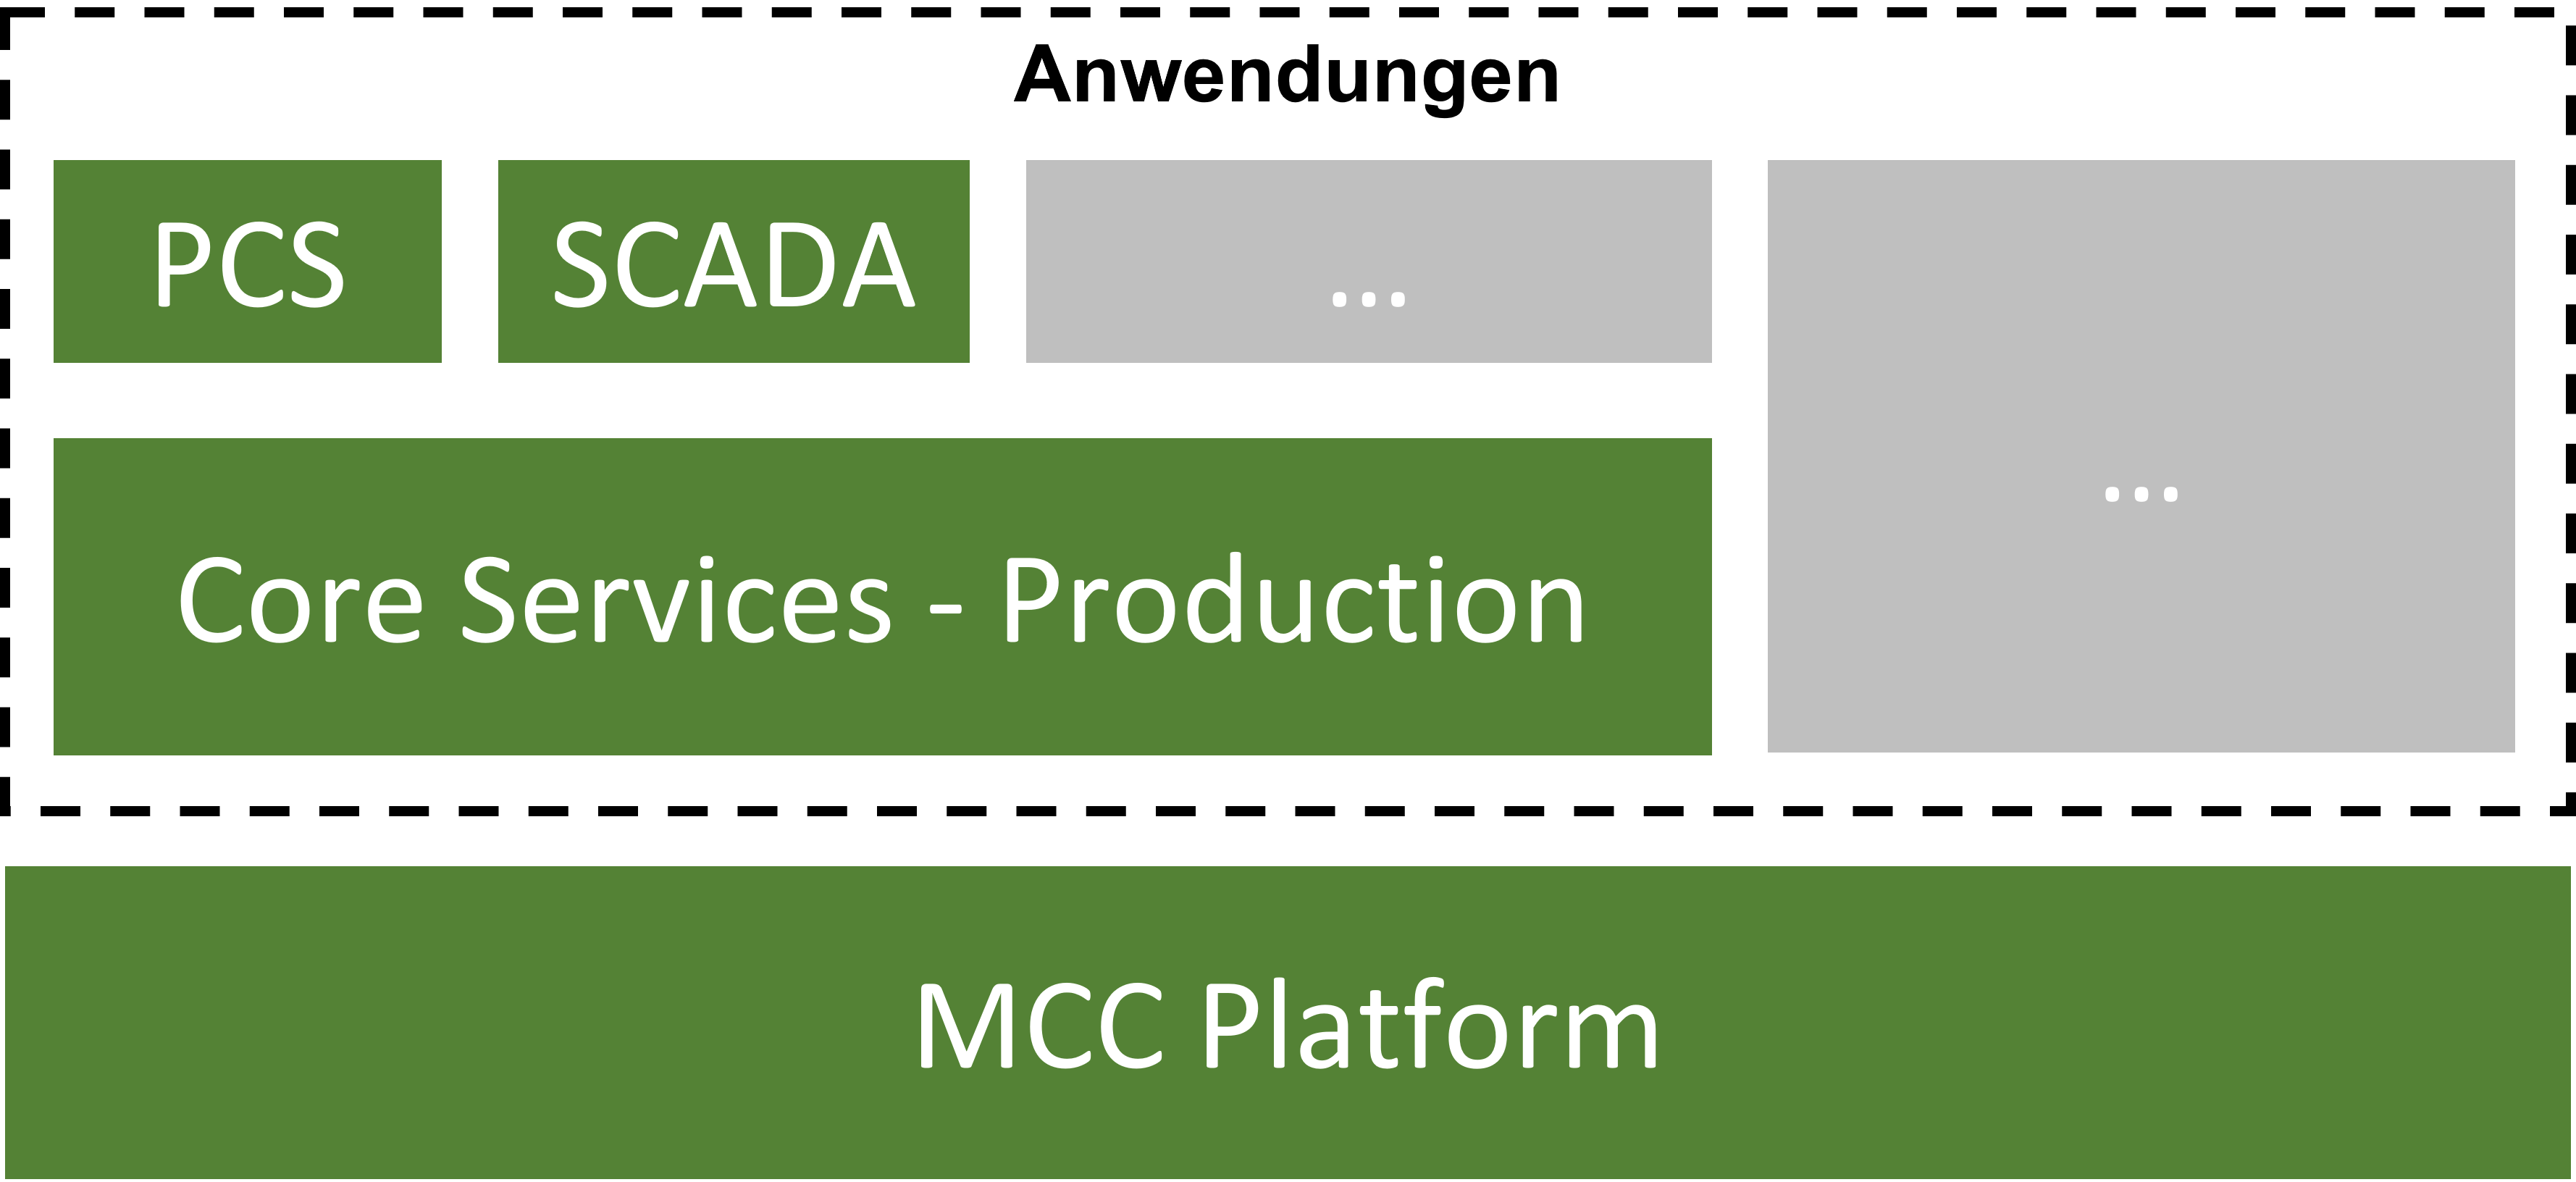
\includegraphics[width=0.7\linewidth]{images/MCC_Layer.png}
    \caption{Übersicht der verschiedenen Layer von MCC}
    \label{fig:mcc_layer}
\end{figure}

Im Folgenden werden die verschiedenen Schichten mit den darin enthaltenen Funktionalitäten abstrahiert erläutert.

\subsection{MCC Platform\label{subsec3.1.1:Unterunterpunkt-1}}

Die Schicht \glqq MCC Platform\grqq{} fungiert als Rahmenschicht für die Anwendungsentwicklung und stellt die Grundfunktionen für die Erstellung und das Betreiben der Anwendungsschichten zur Verfügung.

Zu den Grundfunktionalitäten zählen unteranderem die Themen:

\begin{description}
    \item[Internationalisierung:]\hfill \\
    Um mit einer Software auch eine internationale Kundschaft zu bedienen, ist es erforderlich die Themen Lokalisierung und Internationalisierung zu bedenken. Hierbei geht es darum, mit den länderspezifischen Formaten für Daten und Zahlen und mit unterschiedlichen Zeitzonen umgehen zu können. Auch die Übersetzung der Texte in die jeweilige Sprache wird unter dem Thema Internationalisierung berücksichtigt.
    
    \item[Migrations-API:]\hfill \\
    Aufgrund der späteren Weiterentwicklung der Module kann es bei neuen Versionen dazu kommen, dass sich die Strukturen der Daten in den Datenbanken geändert haben. Bei der Aktualisierung der Module müssen deswegen die bestehenden Daten in den Datenbanken bezüglich der neuen Struktur migriert werden.

    Durch die Umsetzung einer Migrations-API wird nun für jedes Modul eine versionierte Liste mit allen inkrementellen Migrationen abgespeichert. In Kombination mit einem Protokoll, über bereits durchgeführte Migrationen, kann so eine automatische Ausführung der Migration gewährleistet werden.

    \item[Security:]\hfill \\
    Produktionsleitsysteme, wie \glqq E-MES\grqq{}, haben vermehrt einen komplexen Funktionsumfang, welcher bei falscher Bedienung zu hohen Kosten oder Beschädigungen der Anlage führen kann. Aus diesem Grund ist es erforderlich den Zugriff auf bestimmte Aktionen nur für fachkundiges Personal zugänglich zu machen. So können ganze Funktionen für bestimmte Benutzergruppen entweder gesperrt oder durch Weglassen von Bedienelementen angepasst werden.

    Beim Thema \glqq Security\grqq{} geht es demnach um die Authentifizierung und Autorisierung der Benutzer. Neben der Umsetzung von verschiedenen Authentifizierungsmöglichkeiten, müssen den Benutzern die individuellen Rechtepakete zugeordnet werden.

    % Durch die Verfolgung der Benutzerinteraktionen entstehen Prüfpfade. Wer hat was falsch gemacht?

    \item[Streaming Base:]\hfill \\
    Der Austausch von Nachrichten zwischen Microservices wird über Kafka-Topics des Message Brokers \glqq Apache Kafka\grqq{} koordiniert. Der funktionale Ablauf der Nachrichtenweitergabe besteht dabei grundsätzich aus drei Schritten:

    \begin{itemize}
        \item \textbf{Konsumieren} der Nachrichten aus teils mehreren Kafka-Topics
        \item \textbf{Verarbeiten} der Nachrichten (Interaktionen mit den persistenten Speichern oder mit anderen Microservices)
        \item \textbf{Produzieren} der Nachricht an teils mehrere Kafka-Topics
    \end{itemize}

    Unabhängig der späteren Geschäftslogik wird in der \glqq Streaming Base\grqq{} die Kernimplementierung für den Nachrichtentransport implementiert.
    
    % \item[Activity Engine:]\hfill \\
    % Text

    % \item[Entity Model:]\hfill \\
    % Text

    % \item[Software Dokumentation:]\hfill \\
    % Text

\end{description}

Für den Kontext einer Suchfunktionalität sind die meisten Funktionen nicht relevant, da ein Benutzer mit diesen Funktionen nicht direkt interagiert. Zum Beispiel soll die Funktions- und Arbeitsweise der \glqq Streaming Base\grqq{} dem Benutzer verborgen bleiben.

Geeignet für den Kontext einer Suchfunktionalität sind die Objekte und Informationen aus dem \glqq Security\grqq{} - Modul. Dabei kann zum Beispiel nach den unterschiedlichen Benutzerrollen, den damit verbundenen Rechtepaketen oder diversen Benutzerrechten gesucht werden. So kann durch die Suche nach einem Benutzernamen auch die jeweiligen Rechtepakete gefunden werden und durch die Verwendung eines Sicherheitsaudits, können die Aktivitäten nachverfolgt werden.

% Soll die Online-Dokumentation mit in die Platform?

\subsection{Core Services - Production\label{subsec3.1.2:Unterunterpunkt-2}}

Aufbauend auf den Grundfunktionen der \glqq MCC Platform\grqq{}, welche für den Betrieb einer auf Microservices basierenden Architektur benötigt werden, stellt die \glqq Core Services\grqq{} - Schicht die Grundfunktionen für eigentliche Anwendung zur Verfügung. Im Umfeld von Produktionsanlagen werden Grundfunktionen für die anwendungsspezifischen Schichten \glqq PCS\grqq{} und \glqq SCADA\grqq{} definiert. Oftmals handelt es sich dabei um Funktionen, welche von mehreren darüber liegenden Schichten verwendet werden.

Im Falle des Funktionsumfangs des Produktionsleitsystems \glqq E-MES\grqq{} handelt es sich in dieser Schicht um Funktionen, welche für die übergeordneten Schichten \glqq PCS\grqq{} und \glqq SCADA\grqq{} von Nutzen sind.

Zu den Funktionen zählen zum Beispiel die folgenden Funktionalitäten:

\begin{description}

    \item[Shift Model:]\hfill \\
    Dem Schichtenmodel sind Funktionalitäten für das Anlegen und Verwalten von Schichten zugeordnet. 

    \item[Asset Model:]\hfill \\
    Text

    \item[Document Management:]\hfill \\
    Text

\end{description}

\subsection{SCADA\label{subsec3.1.3:Unterunterpunkt-3}}

Text

% Bei \gls{scada} geht es um die Überwachung und Steuerung von automatisierten Fertigungen. Dabei werden Daten von Maschinen und Sensoren empfangen und somit deren Zustand überwacht. Sammelt man diese Daten, kann man eine zeitliche Statistik über die verschiedenen Maschinen und Sensoren anfertigen und so einen Stillstand der Anlage durch frühzeitige Erkennung von Unregelmäßigkeiten verhindern.

% Aus SCADA-Sicht hat man zwei Möglichkeiten auf die Anlage zu schauen.

% \begin{description}
%     \item[Elektrische/Technische Sicht:]\hfill \\
%     Jene Sicht ist vor allem für die Mitarbeiter sinnvoll, welche direkt an den Maschinen arbeiten. Entweder bei der Steuerung der Maschinen oder deren Wartung. Hierbei ist jeder Maschine und jedem Sensor eine eindeutige anlageninterne Codierung zugeteilt.

%     Zum Beispiel => \textbf{T1C041:Visu.P11.1CI1.States.Automatic.Value}

%     Ein Mitarbeiter kann mithilfe der Codierung direkt heraus lesen, in welchem Bereich der Anlage beziehungsweise in welchem Schaltschrank und an welcher SPS die Maschine oder der Sensor angeschlossen ist. So fällt es dem Mitarbeiter leichter Fehler zu finden und die Anlage zu warten.

%     \item[Asset Sicht:]\hfill \\
%     Eine Möglichkeit ist es die Anlage als Assets zu sehen. Hierbei kann der Begriff "Asset" von den einzelnen Maschinen und Sensoren bis hin zur kompletten Anlage reichen. Im Gegensatz zur elektrischen Sichtweise auf die Anlage, können Assets auch gruppiert werden. Es ist zum Beispiel nicht immer notwendig auf der Ebene der einzelnen Maschinen und Geräte zu interagieren. Die Notwendigkeit den Zustand von zum Beispiel einem hydraulischem Ventil zu erfassen ist im Falle der Wartungsdokumentation gerechtfertigt. Jedoch aus Sicht eines Mitarbeiters, der einen großen Teil der Anlage überwachen und steuern muss, ungeeignet.

%     So ist es hilfreich die Assets nach physikalischen Standorten zu gruppieren. So können zum Beispiel verschiedene Antriebsmotoren und Sensoren als Rollenbahn zusammengefasst werden und dem Mitarbeiter als ein zusammengefasstes Asset dargestellt werden. Die Gruppierungen in dem Sinne immer gröber werden. So können mehrere Rollenbahnen Bestandteil einer Bearbeitungsstation sein. Und mehrere Bearbeitungsstationen können zu Anlagen-Bereichen gruppiert werden. Die dadurch entstandene Hierarchie von Assets kann den kompletten Aufbau der Produktionsanlage widerspiegeln.

%     Zwischen den Assets gibt es jedoch nicht nur die hierarchischen Beziehungen. So kann es sein, dass mehrere Geräte am selben Bedienfeld angeschlossen sind und darüber eine Beziehungen zueinander haben. Auch eine Gruppierung nach Schaltschränken für die Stromversorgung kann vorkommen. Eine weitere Beziehung zwischen den Assets sind die Materialflüsse, welche beschreiben, wie Produktionseinheiten durch die Produktionsanlage bewegt werden können. Es gibt demnach verschiedene Arten von Beziehungen zwischen Assets, welche auf physikalischen Verbindungen, wie Zusammensetzung oder Stromversorgung oder auf logischen Verbindungen, wie Materialflüssen beruhen können.
% \end{description}

% Im SCADA Bereich von E-MES lassen sich nun verschiedene Objekte herausfiltern, nach welchen mithilfe einer Suchfunktionalität gesucht werden kann.

% Durch die hierarchische Aufteilung der Anlage in verschiedene Assets, ist eine Suche nach den Assets ein auftretender Use-Case und sollte durch die neue Suchfunktionalität abgedeckt werden. So kann ein Mitarbeiter zum Beispiel nach den Begriffen "Lackierbereich", "Trockenofen" oder "Rollenbahn" suchen und bekommt eine Auswahl an Funktionen angeboten, welche anhand der Assets ausgeführt werden können. Sollte demnach ein Asset mit der Bezeichnung "Rollenbahn" im System zu finden sein, sollen dem Mitarbeiter Funktionalitäten, wie die Anzeige von Fehlermeldungen (Alarming) und Auswertung von Prozesswerten (Trending) angeboten werden. Auch die Suche nach Schaltschränken oder Pultbereichen kann durch die hierarchische Asset Abbildung realisiert werden.

% Neben der Verwendung der Assets kann auch nach den technischen beziehungsweise elektrischen Bezeichnungen der Maschinen und Sensoren gesucht werden. So kann ein Mitarbeiter, welcher lediglich die Codierungen zur Hilfe hat trotzdem nach zum Beispiel letzten Warnungen oder nach einer Auswertung der gemessenen Werte suchen. Auch eine Informationsgewinnung im Bezug zur Zugehörigkeit der Maschine oder des Sensors zu Anlagenbereichen, Pultbereichen oder Schaltschränken kann im Interesse eines Mitarbeiters sein, welcher lediglich eine Codierung einer Maschine oder eines Sensors zur Verfügung hat.

% Im Grund kann man nach folgenden Objekten suchen:

% \begin{itemize}
%     \item Maschinen/Sensoren (durch deren Codierung)
%     \item Assets
%     \item Pultbereiche
%     \item Schaltschränke
% \end{itemize}

\subsection{PCS\label{subsec3.1.4:Unterunterpunkt-4}}

Text

% Bei \gls{pcs} geht es um die Aufbereitung der Produktionsaufträge für die jeweilige Anlage. Hierfür können Mitarbeiter der Anlage neue Produktionsaufträge einspeisen, welche anschließend durch die Bereitstellung von Templates zu entsprechenden Arbeitsschritten umgeformt werden. Auch ist das Vordefinieren von sich ständig wiederholenden Arbeitsschritten möglich. Dabei wird festgelegt, wann, wo und welcher Arbeitsschritt mit welchem Bauteil und passendem Warenträger ausgeführt werden muss. Mithilfe solch einer Planung, kann eine Koordination der Arbeitsstationen mit den Aufträgen stattfinden und Stillstände einzelner Anlagenbereiche werden minimiert.

% Ein weiterer Use-Case ist die Aufzeichnung von Produktionsdaten bezüglich den einzelnen Aufträgen. So kann beispielsweise vermerkt werden, wie Dick oder Lange eine Lackierung auf dem Werkstück XY appliziert wurde. Im Nachgang können dann, zu jedem Werkstück oder auch Arbeitsauftrag, sämtliche Produktionsdaten nachvollzogen werden.

% Für eine Suchfunktionalität gibt es im PCS-Umfeld verschiedene Anwendungsfälle. Die Aufträge, welche von der Anlage abgearbeitet werden haben in der Regel eine eindeutige Identifikationsnummer. Wenn ein Mitarbeiter solch eine Identifikationsnummer in das Suchfeld eingibt, erwartet dieser eine Auflistung an Funktionen, welche ich auf den jeweiligen Produktionsauftrag anwenden kann. Zum Beispiel möchte ich einsehen können, welchen Status mein Auftrag gerade hat und welche Arbeitsschritte noch ausstehen. Auch möchte man eventuell gezielt nach verschiedenen Warenträgern suchen, um herauszufinden, welche Aufträge mit dem Warenträger transportiert worden sind.

% Im Grund kann man nach folgenden Objekten suchen:

% \begin{itemize}
%     \item Bauteile
%     \item Aufträge
%     \item Warenträger
%     \item Maschinen
%     \item Arbeitsschritte
% \end{itemize}

\section{Umfang einer Volltextsuche\label{sec3.2:Unterunterpunkt-2}}

Text

\section{Umfang einer facettierten Suche\label{sec3.3:Unterpunkt-3}}

Text

\section{Umfang einer facettierten Volltextsuche\label{sec3.4:Unterpunkt-4}}

Text

\section{Umfang einer semantischen Suche\label{sec3.5:Unterpunkt-5}}

Text